\chapter{Methods}

\begin{keytakeaway}
    We describe the three primary modeling techniques used in this study: \textbf{Linear Mixed-Effects regression}, \textbf{Bayesian Ridge regression}, and \textbf{CatBoost regression}. We chose to explore these models because they are \textbf{well-suited for the analysis of longitudinal data}, they provide a good balance between model complexity and generalizability, and they are \textbf{particularly effective for handling categorical variables with a high number of levels}.
\end{keytakeaway}

\section{Data Considerations}
Throughout our analysis, our primary focus is on the Next-Year Decarbonization Rate, a continuous variable. Our goal is to identify key predictors and assess their impact on this response within a multiple timeseries framework, where each firm's annual reports represent individual yearly observations. With an average data span of just 6 years, the dataset is too small for the application of deep learning or traditional single-firm timeseries models. Therefore, our strategy involves employing models that allow us to borrow strength across firms and industries while ensuring the outcomes remain interpretable. Moreover, we must navigate the high dimensionality of our data, which includes 130 predictors, among which are categorical variables with a vast number of levels.

I have chosen Mixed-Effects models as they are exceptionally suitable for our longitudinal data analysis. This approach enables us to introduce random intercepts for categorical variables with extensive levels, specifically \textit{Id}, \textit{Country}, \textit{Industry}, and \textit{Continent}. By doing so, we can effectively borrow strength across these dimensions. Mixed-Effects models offer a balance between interpretability and the necessity for manual tuning. In our process of determining the most significant predictors, we will, in Chapter \ref{chap:chapter4}, proceed to develop models of increasing complexity. We start by establishing the optimal panel structure, then methodically incorporate groups of CDP predictors by their significance, including Emission Figures, Investment, Incentives, Risks, and Opportunities. Each group will be added to the model iteratively, thus building increasingly complex models. 

This step-by-step model building approach allows us to analyze key relationships to gather insights from CDP data and to ensure that those relationships are both logical and intuitive. As you will see, we will find surprisingly coherent and consistent relationships, indicating that the CDP data can be highly informative of future decarbonization efforts. At every step, we will advance the most relevant predictors to subsequent models to prevent overfitting. Our model selection and refinement process is guided by the Akaike Information Criterion (AIC) and the Bayesian Information Criterion (BIC), which serve as tools to compare the statistical quality of our models.

\section{Mixed Effects Models}

The main statistical method used in this study is the linear mixed-effects model (LMM) implemented via the R package lme4 \cite{lmer}. LMMs are a generalization of linear regression models that allow for the inclusion of both fixed and random effects. Fixed effects are the parameters of interest, while random effects are used to account for the correlation between observations within the same group. Mixed-effects models are particularly useful for longitudinal data, where repeated measurements are taken on the same subjects over time. In our case, the repeated measurements are the yearly company CDP reports, given that the same companies report their emissions over multiple years. Furthermore, we use random effects for categorical variables that have a high number of levels, such as countries, industries, companies and continent. This approach allows the model to capture the variability in the data due to these categorical variables, while also reducing the risk of overfitting and improving the generalizability of the model. As Bates explains, mixed-effects models are also known as \textit{multilevel} models because the random effects represent levels of variation in addition to the pre-observation noise term that is incorporated in common statistical models such as linear regression models, generalized linear models, and nonlinear regression models \cite{bates}. Furthermore, there have been many successful applications of mixed-effects models in problems with similar settings, such as the work of Maruotti et al. who use bivariate bi-dimensional mixed-effects regression model and effectively captures heterogeneity in CO2 emissions and growth across OECD countries from 1990 to 2018 \cite{Maruotti2023CO2}, or the work of Zanin et al. who assessed the functional relationship between CO2 emissions and economic development using an additive mixed model approach \cite{zanin}.

\subsection{Model Specification}
Let's consider a simple linear mixed-effects model having next year decarbonization rate as a response with an intercept, a single fixed effect, and a single random intercept. In our case, the fixed effect will be the year of the report, and the random effect will be the company. Let $y_{ij}$ be the response variable at the $i$-th year for the $j$-th company, let $x_{ij}$ be the fixed effect at the $i$-th year for the $j$-th company, and let $z_{ij}$ be the random effect at the $i$-th year for the $j$-th company. The linear mixed-effects model can be written as \cite{duke_sta216_lecture}:
\begin{align}
    Y_{ij}| \alpha_j &= \alpha_j + \beta_0 + \beta_1 X_{ij} + \epsilon_{ij} \\
    \alpha_j &\sim N(\mu_{\alpha}, \sigma^2_{\alpha}) \\
    \epsilon_{ij} &\sim N(0, \sigma^2) \\
    i &= 1, 2, ..., n_j \\
    j &= 1, 2, ..., J
\end{align}
Where $J$ is the number of companies, $n_j$ is the number of years for the $j$-th company, $\alpha_j$ is the random intercept for the $j$-th company, $\mu_{\alpha}$ is the mean of the random intercepts, $\sigma^2_{\alpha}$ is the variance of the random intercepts, $\beta_0$ is the fixed intercept, $\beta_1$ is the fixed effect, and $\epsilon_{ij}$ is the error term. Note how the corresponding OLS model would require to control for the company fixed effects by including a dummy variable $D_j$ for each company:
\begin{align}
    Y_{ij} &= \beta_0 + \beta_1 X_{ij} + \sum_{j=1}^{J} \alpha_j D_j + \epsilon_{ij}
\end{align}
In the ordinary least squares (OLS) model, we introduce a separate parameter for each of the $J$ groups which leads to the estimation of $J$ additional coefficients. This can be inefficient, particularly when $J$ is large. In contrast, in the mixed-effects model we introduce only two additional parameters for the random effects: $\sigma^2_{\alpha}$, which represents the variance of the random intercepts across groups, and $\sigma^2_e$, which represents the residual variance within groups. These parameters are estimated from the data using the Restricted Maximum Likelihood (REML) method \cite{bates}. REML is particularly effective because it corrects for the potential bias introduced by estimating fixed effects alongside the variance components. This approach enhances model efficiency and reduces the risk of overfitting, especially in scenarios with a large number of groups. Once the variance components $\sigma^2_{\alpha}$ and $\sigma^2_e$ are estimated, the model employs a process known as \textit{shrinkage} to compute the individual random effects (intercepts) for each group. Shrinkage is a regularization technique that adjusts the individual group estimates, pulling them towards a central value, typically towards the overall population mean, which in the context of many mixed models is assumed to be zero \cite{bates}. This shrinkage effect is governed by the relative sizes of $\sigma^2_{\alpha}$ and $\sigma^2_e$. Specifically:
\begin{itemize}
    \item If $\sigma^2_{\alpha}$ is large compared to $\sigma^2_e$, it indicates significant variability among the groups. Thus, the random intercepts for each group are allowed to deviate more from the overall mean, reflecting the distinct characteristics of each group.
    \item Conversely, if $\sigma^2_{\alpha}$ is small relative to $\sigma^2_e$, it suggests that the groups are not markedly different from each other. As a result, the random intercepts are more heavily shrunk towards the central value, reducing the differences among group intercepts.
\end{itemize}
This approach allows the mixed-effects model to balance between capturing the unique attributes of each group and maintaining model parsimony and generalizability, making it particularly useful when dealing with a large number of groups.

\subsection{Extension to Multiple Fixed Effects and Random Slopes}
The linear mixed-effects model can be extended to include multiple fixed effects and random slopes. Let $X$ be a $n \times p$ matrix of fixed effects, where $n$ is the number of observations and $p$ is the number of fixed effects. Let $Z$ be a $n \times q$ matrix of random effects, where $q$ is the number of random effects. The linear mixed-effects model can be written as \cite{duke_sta216_lecture}:
\begin{align}
    Y|\gamma &= X\beta + Z\gamma + \epsilon \\
    \epsilon &\sim \mathcal{N}(\mathbf{0}, \sigma^2I) \\
    \gamma &\sim \mathcal{N}(\mathbf{0}, \sigma^2\Sigma) \\
    \gamma &\perp \epsilon
\end{align}
We followed the notation of Baayen et al. \cite{BAAYEN2008390}, where $Y$ is a $n \times 1$ vector of response variables, in our case \textit{Next Year Decarbonization Rate}, $\beta$ is a $p \times 1$ vector of all the CDP predictors that we test in various iterations, $\gamma$ is a $q \times 1$ vector of random effects, in our case \textit{Id}, \textit{Country}, \textit{Continent}, and \textit{Industry}, $\epsilon$ is a $n \times 1$ vector of error terms, $\Sigma$ is a $q \times q$ covariance matrix of random effects, and $I$ is the identity matrix. The covariance matrix $\Sigma$ is estimated from the data using the REML method in the lmer package \cite{bates}.



% Using Kenward-Roger or Satterthwaite approximations for evaluating significance in linear mixed-effects models in R provides more conservative results than likelihood ratio tests and t-as-z, especially for smaller sample sizes \cite{Luke2016Evaluating}.

\section{Bayesian Ridge Regression}
\subsection{Considerations}
The choice to deploy a Bayesian Ridge regression model specifically addressess the main shortcoming of the mixed-effects model, which is the \textbf{lack of regularization and variable selection}. While I manually selected optimal variables for Mixed-Effecs models, ensuring that the model was not overfitting, the Bayesian Ridge regression model automatically selects the most relevant variables and regularizes the coefficients. This is particularly useful in the context of our study, where we have a large number of CDP predictors and we are interested in identifying the most important ones. Furthermore, the Bayesian Ridge regression model provides confidence intervals for the coefficients, which can be highly informative and lead to interesting interpretations. Bayesian Ridge regression has been successfully applied in various fields, such as Forecasting COVID-19 outbreak progression by Saqib \cite{saqib} or to predict Overall Equipment Effectiveness performance in corporate setting by Imane et al. \cite{imane}

Bayesian techniques can be used to include regularization parameters which is not set in a hard sense but tuned to the data. This can be done by introducing uninformative priors over the hyper parameters of the model \cite{scikit-learn, mackay_bayesian_1992}. The $l_2$ regularization parameter used in Ridge regression is equivalent to finding a maximum a posetiori estimation under a Gaussian prior over the coefficients $w$ with precision $\alpha^{-1}$ \cite{scikit-learn}. Effectively, we can use a Bayesian method to replicate regularization, with the advantage of being able to build confidence intervals for the coefficients. Using this model makes sense given our objectives, as we have a large number CDP of features and we are interested in finding the most relevant ones, while at the same time avoiding overfitting and building an overly complex model. Furthermore, a bayesian approach is a great complement to the mixed-effects model, as it provides confidence intervals for the coefficients, which can be highly informative in the context of our study. We will report the specification presented by Tipping \cite{tipping} which is implemented in the scikit-learn library \cite{scikit-learn}.

\subsection{Model Specification}
Consider a data set of input-target pairs $\{\mathbf{X_n}, t_n\}^N_{n = 1}$ we follow the standard probabilistic formulation and assume that targets are samples from the model with additive noise: 
\begin{align}
    t_n = y(\mathbf{x}_n, \mathbf{w}) + \epsilon_n
\end{align}
where $\epsilon_n$ iare independent samples from some noise process which is assumed to be mean-zero Gaussian with variance $\sigma^2$ \cite{tipping}. Therefore we have:
\begin{align}
    p(t_n|\mathbf{x}) = \mathcal{N}(t_n|y(\mathbf{x}_n), \sigma^2)
\end{align}
the notation specifies a Gaussian distribution over the target variable $t_n$ with mean $y(\mathbf{x}_n, \mathbf{w})$ and variance $\sigma^2$. Assuming independence of $t_n$, we can write the likelihood of the complete data set as \cite{tipping}:
\begin{align}
    p(\mathbf{t}| \mathbf{w}, \sigma^2) &= (2 \pi \sigma^2)^{-\frac{N}{2}} \exp\left\{-\frac{1}{2\sigma^2}||\mathbf{t} - \Phi \mathbf{w}||^2\right\} \\
    t &= (t_1, t_2, ..., t_N)^T \\
    w &= (w_1, w_2, ..., w_N)^T
\end{align}

\noindent Then, we encode a preference of smoother functions by using a zero-mean Gaussian prior over the parameters $\mathbf{w}$, with precision $\alpha$ \cite{tipping}:
\begin{align}
    p(\mathbf{w}|\alpha) &= \prod_{i = 0}^{N} \mathcal{N}(w_i|0, \alpha^{-1}) \\
\end{align}
where $\mathbf{\alpha}$ is a vector of $N + 1$ hyperparameters. Note that there is an individual hyperparameter associated independently with every weight. To complete the specification of this hierarchical model, we define hyperparameters over $\mathbf{\alpha}$ as well as the final remaining hyperparameter $\sigma^2$, we do so by using Gamma priors\cite{tipping}:
\begin{align}
    p(\alpha_i) &= \text{Gam}(\alpha_i|a, b) \\
    p(\beta) &= \text{Gam}(\beta|c, d) \\
    \beta \equiv \frac{1}{\sigma^2} \\
    \text{Gam}(\alpha|a, b) &= \Gamma(a)^{-1} b^a \alpha^{a - 1} \exp(-b\alpha)
\end{align}

\subsection{Non informative Priors}
The key aspect of the model is that we intentionally make these priors non-informative by fixing their parameters to small values e.g. $a = b = c = d = 10^{-4}$ \cite{tipping}. The incredibly interesting aspect of such approach is that this formulation of priors is a type of \textit{automatic relevance determination} \cite{MacKay1996} where a broad prior over the hyperparameters allows the posterior to concentrate at very large values of some of those $\alpha$ values, with the advantage that the associated posterior weights probability will be concentratd around zero, effectively eliminating the corresponding inputs and deeming them as irrelevant, thus providing a form of automatic feature selection \cite{tipping}. 


\section{CatBoost Regression}
To achieve maximum predictive accuracy, and address the high dimensionality of the data, I chose to use the CatBoost algorithm. CatBoost is a state-of-the-art machine learning algorithm developed by Yandex, specifically designed to efficiently handle categorical variables \cite{prokhorenkova2018catboost}. This algorithm is particularly useful in our case as we have multiple important categorical predcitors, namely \textit{Id}, \textit{Country}, \textit{Industry}, and \textit{Continent} which are crucial to the analysis but at the same time have a high number of levels. If we were to one-hot encode these categorical variables, we would end up with a large number of features, which would make the model more prone to overfitting and would require a larger dataset to train effectively, which we do not have. This is one of the key reasons of why we previously used mixed-effects models Therefore, the CatBoost algorithm is particularly well suited for forecasting the decarbonization rate of companies based on the CDP data as it allows to use the whole dataset for training and to handle categorical features efficiently. Additionally, there is ample literature demostrating that CatBoost is a state-of-the-art algorithm for multi-source data, which is precisely the case of our study. As Pan et al. explain, the CatBoost model is particularly suited for multi-source heterogeneous data, outperforming popular machine learning algorithms like random forest and gradient boosting decision tree \cite{Pan2020Data}. We find similar results in our own study, as we will show in chapter \ref{ch:finding-the-best-model}. Additionally, CatBoost has been successfully used in multiple emission forecasting  settings, such as in the research of Marco et al. to forcast carbon dioxide emissions of light-duty vehicles \cite{marco} or in the work of Bai to predict emission characteristics in low carbon biofuel-hydrogen dual fuel engines \cite{bai}.

\subsubsection{Handling Categorical Features}

CatBoost transforms categorical features into numerical values using an efficient strategy which reduces overfitting and allows to use the whole dataset for training \cite{dorogush2018catboost}. 
In particular, a random permutation of the dataset is performed and for each example the algorithm computes the average label value for the example with the same category value placed before the given one in the permutation \cite{dorogush2018catboost}. Let $\sigma = (\sigma_1, \sigma_2, ..., \sigma_n)$ be the permutation of the dataset, then $x_{\sigma_p, k}$, the predictor corresponding to observation $k$ in partition $\sigma_p$ is substituted with:
\begin{align}
    \frac{\sum_{i=1}^{p-1} [x_{\sigma_i, k} = x_{\sigma_p, k}] \cdot y_{\sigma_j} + a \cdot P }{\sum_{i=1}^{p-1} [x_{\sigma_i, k} = x_{\sigma_p, k}] + a}
\end{align}
\noindent finally, the algorithm uses the transformed variable to build the decision tree \cite{dorogush2018catboost}.

\subsubsection{Gradient Boosting Framework}

\begin{figure}[H]
    \centering
    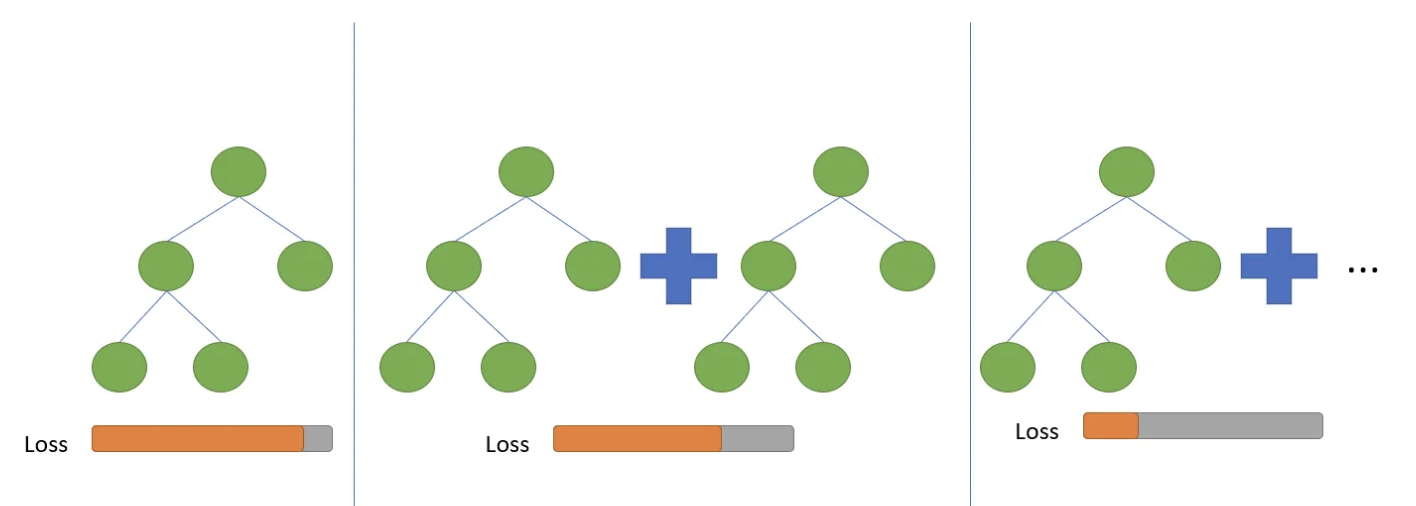
\includegraphics[width=0.7\textwidth]{figures/gradient_boosting_v2.png}
    \caption{Gradient boosting. Adapted from \cite{Yenigun2022}}
    \label{fig:catboost}
\end{figure}

In this section I will briefly highlight Catboost's unique features. The CatBoost algorithm is based upon oblivious decision trees, which are trees that make decisions based on only one feature at a time \cite{dorogush2018catboost}, this design ensures that the threes are balanced and less prone to overfitting. At the same time, using oblivious trees allows for a more efficient implementation and faster execution speed. In Ordered boosting mode \cite{dorogush2018catboost}, Catboost usues supporting models $M_{r,j}$ to make predicitons based on peromutations of training samples. Note that the random permutation $\sigma_r$ chosen for each tree-building iteration are the same used to calculate the Target Statistics for categorical features embeddings. Finally, the implementation of Catboost I will be using in the following chapters uses \textit{l2} regularization on the leaf values of the trees to prevent overfitting \cite{dorogush2018catboost,prokhorenkova2018catboost}. For a general overview of gradient boosting, the literature is vast and I suggest to go over the Survey from He et al. \cite{he2019gradient} or the overview of XGBoost, a popular tree bosting system, by Chen et al. \cite{Chen_2016}. 




% \section{Bayesian Ridge Regression}

% \section{CatBoost Regression}

% \section{Neural Networks}
